\documentclass{article}
\usepackage[utf8]{inputenc}
\usepackage[hidelinks]{hyperref}
\usepackage{graphicx}


\title{Domande Architectures For Big Data}
\author{Marco Dalla Bà e Marco Incerti}
\date{January 2022}

\begin{document}

\maketitle
\tableofcontents

\section{Enterprise Architecture}
\subsection{Describe the link between building architecture and software architecture? What are common concepts between this two subjects?}

La building architecture è l’arte o la pratica di progettare e costruire strutture, specialmente le abilitabili, utilizzando forme e strutture coerenti. Allo stesso la software architecture è l’arte o la pratica di organizzare e scegliere lo stile che incapsula e connette le varie componenti software. 
Altri punti in comune presi dalla building architecture e proiettati nella software architecture sono:
\begin{itemize}
    \item Visioni multiple
    \item Stili architetturali
    \item Stili e materiali
\end{itemize}

Un architetto edile lavora con il cliente attraverso una serie di viste diverse in cui viene enfatizzato un aspetto particolare dell'edificio.
Ad esempio, ci sono prospetti e planimetrie che forniscono rispettivamente le viste esterne e le viste "top-down".
Le viste di prospetto possono essere integrate da disegni contestuali o anche modelli in scala per fornire al cliente l'aspetto dell'edificio nel suo contesto.
Si hanno anche differenti stakeholder; Ogni prospettiva non è solo una questione di diverso livello di dettaglio. È collegato a diverse nature e responsabilità.
Il proprietario ha bisogno dell'edificio per uno scopo specifico. Lui non sa come, ma sa perfettamente perché.
L'architetto ha bisogno di progettare e formalizzare qualcosa che si adatti perfettamente alle esigenze del proprietario, per pianificare il cosa.
Il Costruttore deve progettare come ciò che verrà costruito rispettando le leggi naturali e i vincoli tecnologici.

Allo stesso modo nella software architecture diverse tipologie di utenti utilizzeranno l'Architettura del Software: ognuno di loro avrà bisogno di un punto di vista specifico.
Uno sviluppatore Full Stack deve sapere come scrivere codice all'interno dell'architettura mentre un Data Scientist dove sono i dati di cui ha bisogno.

La building Architecture sfrutta diversi STILI architetturali;
Descrittivamente, lo stile architetturale definisce una particolare codificazione degli elementi di design e delle disposizioni formali.
Prescrittivamente, lo stile limita i tipi di elementi di design e le loro disposizioni formali.
Cioè, uno stile architettonico vincola sia gli elementi di design che le relazioni formali tra gli elementi di design.

Allo stesso modo nella software architecture, lo stile architetturale racchiude decisioni importanti sugli elementi e sottolinea importanti vincoli su di essi e sulle loro relazioni.
Possiamo usare lo stile architetturale sia per vincolare l'architettura che per coordinare gli architetti che collaborano.
Inoltre, lo stile incarna quelle decisioni che subiscono l'erosione e il drift: l'enfasi su di esso come vincolo dell'architettura fornisce visibilità a determinati aspetti dell'architettura in modo che le violazioni di quegli aspetti e l'insensibilità ad essi siano più evidenti.

L'architettura classica unisce STILE e MATERIALI
I materiali hanno determinate proprietà che vengono sfruttate per fornire uno stile particolare. Si possono combinare usi strutturali ed estetici dei materiali, come quello che si trova nella costruzione di pilastri e travi delle case in stile tudor.
Tuttavia, non si costruisce un grattacielo con pali e travi di legno.
Gli aspetti materiali degli elementi di design forniscono basi sia estetiche che ingegneristiche per un'architettura.

Nella software architecture, la stessa funzione può essere ottenuta utilizzando diversi sottosistemi.
Addestrare una rete neurale Python potrebbe essere la soluzione migliore, mentre mettere in produzione la rete addestrata utilizzando FPGA per costruire fisicamente la rete potrebbe essere una soluzione migliore.

\subsection{Define what “Software Architecture” mean}
Un'architettura software è un insieme di elementi architettonici che hanno una forma particolare.
La forma architettonica è costituita da proprietà ponderate e
relazioni.
Una parte soggiacente, ma integrante, di un'architettura è la logica delle varie scelte fatte nella definizione di un'architettura

\subsection{The Project Execution pyramid (slide 23 - Lesson 002 – Architecture 101)}
\begin{enumerate}
    \item \textbf{Requisiti:} Determinazione delle informazioni, del trattamento e delle caratteristiche di tali informazioni e del trattamento necessarie all'utente del sistema
    \item \textbf{Architettura:} Selezione degli elementi architettonici, delle loro interazioni e dei vincoli per fornire un quadro in cui soddisfare i requisiti e fungere da base per la progettazione
    \item \textbf{Design:} Modularizzazione e interfacce dettagliate degli elementi progettuali, dei loro algoritmi e procedure, e dei tipi di dati necessari per supportare l'architettura e soddisfare i requisiti
    \item \textbf{Implementazione:} Rappresentazioni degli algoritmi e dei tipi di dati che soddisfano la progettazione, l'architettura e i requisiti

\end{enumerate}
\subsection{What is an abstraction? How an abstraction is created? How can we use this concept when we try to design an Architecture?}
L'essenza dell'astrazione è riconoscere un modello, nominarlo e definirlo, analizzarlo, trovare modi per specificarlo e fornire un modo per invocare il modello con il suo nome senza un intervento manuale soggetto a errori.
Questo processo elimina i dettagli dell'implementazione del modello, riduce l'opportunità di errori materiali e semplifica la comprensione del risultato.
In altre parole, una buona astrazione è ignorare i dettagli giusti al momento giusto.

Un’astrazione caKura proprietà essenziali dei soKo-sistemi più importan* e i modi in cui interagiscono. Inizialmente, i problemi vengono risol* ad hoc; più si accumula esperienza, più si notano soluzioni migliori altre, con un passaggio di folklore che viene passato informalmente da persona a persona. Pian piano, le soluzioni migliori vengono capite meglio e vengono codificate ed analizzate.


Lo sviluppo delle singole astrazioni segue spesso uno schema comune:
\begin{itemize}
    \item In primo luogo, i problemi vengono risolti ad hoc.
    \item Man mano che l'esperienza si accumula, alcune soluzioni funzionano meglio di altre e una sorta di folklore viene trasmesso in modo informale da persona a persona.
    \item Alla fine le soluzioni utili vengono comprese in modo più sistematico, codificate e analizzate.
    \item Questo a sua volta consente un livello di pratica più sofisticato e ci consente di affrontare problemi più difficili".
\end{itemize}
Un'esempio di astrazione è quello utilizzato nello schema ISO/OSI.
\subsection{What are the main pillars of any Software Architectures? Describe each of them with practical example to show the added value}
Le colonne portan* di un’architettura sono:
\begin{itemize}
    \item Essere il framework per la soddisfazione dei requisiti: Funzionali, tecnici e di sicurezza (GDPR)
    \item Essere la base tecnica per il design: indica la strada da seguire per le interfacce dettagliate degli elementi di progettazione, algoritmi, procedure e tipi di dato
    \item Essere la base manageriale per una stima dei costi e della gestione dei processi
    \item Abilitare il riuso di componenti: Stessi componenti, ma con logiche diverse
    \item focalizzarsi sulla centralizzazione: in molti casi rendere un processo centralizzato permette di risparmiare costi a livello di tempo e di gestione (ad esempio è bene che il log tracing sia centralizzato e quindi accessibile da un'unica sorgente (singola fonte di verità) in cui ripescare i vari log non comporti una fase di merge da diverse sorgenti). Nota che questo punto NON va contro il principio di un sistema distribuito, ma consiste nel sottolineare l'importanza di avere un'unica fonte di interesse da/su cui lavorare
    \item Aumentare la produttività e la sicurezza: Individuare punti deboli, porte da aprire, costruire un gateway, nascondere il Data Lake...
    \item Abilitare la possibilità di integrare sistemi aziendali
    \item Abilitare una scalabilità ordinata
    \item Controllare l’esecuzione dei processi soJware (dove)
    \item Evitare handover e lock-in
\end{itemize}
\subsection{What is a design pattern?}
Sono best practices formalizzate e condivise che risolvono problemi comuni. É un template che può essere usato in contesti e situazioni diverse.

\subsection{ETL pattern and evolutions based on Data Lake}
L'ETL pattern è un singolo processo che prende i dati non strutturati, effettua una sorta di elaborazione e salva il risultato in un luogo strutturato. Le informazioni scartate spesso non sono estraibili una seconda volta.

Il data lake è uno spazio di storage praticamente immenso, che permette:
\begin{itemize}
\item La memorizzazione di dati non processati, eterogenei e da qualsiasi fonte (serializzati in oggetti)
\item Dati salvati per sempre
\item Buone performance di reading/writing
\item Schema disponibile on-read
\end{itemize}

E’ basato sull'Object Storage Model, architettura di data storage che gestisce i dati come oggetti. Ogni oggetto contiene dati, metadata (informazioni contestuali) e informazioni tecniche (header).
É basato su una convenzione di nomenclatura, la quale genera un ID univoco per ogni oggetto, ed una strategia di serializzazione condivisa (es JSON). Permette di distribuire dati su più nodi.

Ha cambiato il pattern ETL in ELT, Extract – Load – Transform; infatti, i legacy sistems sono abbastanza costosi e complessi, e l’informazione prodotta e non salvata è persa per sempre. Non c'è ragione dunque per non salvare tutta l’informazione possibile, per effettuare a posteriori qualsiasi trasformazione si voglia (lasciando anche più spazio alle possibilità di analisi effettuabili). Da qui, lo schema on-read.

Si evolve quindi in ELT: Un primo processo prende e carica i dati così come sono, applicando solamente una serializzazione standard (es. Json). Un secondo processo prende queste strutture dati e esegue le trasformazioni richieste.

\subsection{How can we implement the CDC pattern? Pro(s) and Con(s) of each approach}
Insieme di design patterns per determinare i dati che sono cambiati (freschi) e le azioni da intraprendere sui dati cambiati. Riferiti a Log o Registry/Master tables (e sono batch).

\textbf{Invasivi lato Database:}
\begin{itemize}
    \item Timestamp su righe: ok log, critico per registry perché rallenta SELECT, INSERT, UPDATE, DELETE e se non è indicizzato la ricerca è molto lenta.
    \item Numero di versione su righe: come timestamp, ancora peggio in quanto richiede una query interna per trovare il numero massimo di versione.
    \item Indicatore di stato su righe: gravissimi problemi di concorrenza (chi resetta?)
    \item Trigger su tabelle: Problemi di performance, possono diventare ingestibili e hanno problemi di concorrenza (inserire in una tabella lockata mette in pausa l’esecuzione)
\end{itemize}

\textbf{Invasivi lato Applicativo:} Programmazione ad eventi, la responsabilità di propagare i cambiamenti è dell'applicazione. Ogni volta che committa qualcosa, esso deve essere mandato anche al CDC. Problema soprattutto perché l'app potrebbe essere basata su legacy system e potrebbe non garantire proprio questa possibilità.

\textbf{Invasivi lato CPU Database:}
\begin{itemize}
    \item Transaction Log scanners: Leggere e processare alcuni log tecnici del database, individuare i cambiamenti e propagarli al sistema CDC. Non sono generici e non sono aperti.
    \item Log Shipping: Sfruttare un processo automatico di backup del DB per propagare i cambiamenti (in modo incrementale e con tecniche interne non accessibili). Usato soprattutto nelle soluzioni di Disaster Recovery.
\end{itemize}

\subsection{CDC, statefull/stateless and transactionality}
\textbf{Change Data Capture} (CDC) è un insieme di design patterns usati per determinare e tenere traccia dei dati che sono cambiati, in modo che le azioni possano essere eseguite utilizzando i dati modificati.
\newline Per \textbf{stateful} intendiamo la capacità di un sistema di ricordare eventi o interazioni dell'utente precedenti. Mentre, per \textbf{stateless} si intende la capacità di un sistema di rispondere sempre allo stesso modo indipendentemente da qualsiasi stato precedente.
\newline Il \textit{Diff\&Where CDC pattern} che abbiamo visto è \textbf{stateless} poiché si sta leggendo esternamente e ogni volta che viene eseguito, il CDC prende il file \textit{sync.json} e lo aggiorna. Non c'è quindi una storia degli "stati passati". CDC può essere sia stateful che stateless ma è meglio che sia stateless. 
\newline CDC può essere \textbf{transactional}? Per \textit{transactional} si intende che rispetti le proprietà ACID (Atomicity, Consistency, Isolation e Durability), in altri termini che possano essere eseguiti commit e rollback. 
Il Diff\&Where incremental pattern può fallire, dal momento che l'inserimento delle righe nel database e l'aggiornamento del file \textit{sync.json} viene fatto in parallelo. Se l'inserimento delle righe fallisce (comune per l'inserimento di grandi quantità di righe), però, l'aggiornamento del file \textit{sync.json} viene fatto comunque.
Per risolvere questo tipo di problema bisogna fare in modo che CDC diventi transactional. Per fare questo, qunado ci connettiamo a SQL puliamo tutti i file ".tmp" del Data Lake e successivamente, dopo avere preso le nuove righe con "Diff\&Where", eseguiamo sequenzialmente l'inserimento elle righe nel Data Lake e l'aggiornamento del file \textit{sync.json}. Questo pattern viene chiamato \textbf{Move and Rename} ed è basato sull'utilizzo di nomi temporanei, sulla rinomina dei file in una volta sola al termine del processo di scrittura e su uno step finale di pulizia da eseguire all'inizio di ogni "lavoro".

\subsection{Differences between log and registry when we try to implement the CDC pattern}
Per prima cosa definiamo Registry Data Table e Log Data Table. Una \textbf{Log Data Table} è una tabella che registra gli eventi (per esempio, acquisti/vendite di un'azienda), mentre un \textbf{Registry Data Table} è una tabella che descrive le entità che potrebbero cambiare nel corso del tempo (per esempio, la lista dei materiali necessari a produrre qualcosa).
I CDC pattern tradizionali presentano diverse diverse criticità e il modo migliore per risolvere questo problema è utilizzare il \textbf{Diff\&Where incremental pattern}, che è basato su:
\begin{itemize}
    \item Una stategia \textit{"where-like"} per la log table. Ovvero, si sfruttano i timestamps contenuti nella tabella per estrarre solo le righe dove il timestamp è maggiore rispetto all'ultimo timestamp dell'iterazione precedente.
    \item Una stategia \textit{"diff-like"} per la registry table. Viene calcolato un hash per le chiavi (KHASH) e i valori (HASH) della tabella e si confrontano khash e hash in due instanti diversi della tabella per capire se c'è sato un INSERT, un UPDATE o una DELETE (es. in presentazione 004 - slide 23).
\end{itemize}
In questo modo tutti i problemi dei tradizionali patterns sono risolti.

\subsection{What could be used the wrapper pattern for? Why?
Distribute Computation}
L’adapter pattern permette di mitigare l’effetto di Vendor Lock-in in quanto le applicazioni non dipendono direttamente da un servizio esterno, ma comunicano con esso tramite un'interfaccia interna (Wrapper) che espone funzionalità del servizio esterno (e può decidere anche di nascondere alcune funzionalità). In questo modo, nel caso si scegliesse di cambiare fornitore del servizio esterno basterebbe cambiare il codice all'interno dell'Adapter Pattern, senza dover cambiare ogni singola applicazione.
La classe Wrapper permette di chiamare servizi esterni senza esporre direttamente le interfacce di essi, ma bensì e interfacce del Wrapper.


\subsection{What is Map Reduce? When it was first formalized?}
MapReduce è un modello di programmazione proposto in un documento di Google (2003) per semplificare la parallelizzazione dei processi multinodo:
\begin{itemize}
    \item Gli utenti specificano una funzione mappa che elabora una coppia chiave/valore per generare un insieme di coppie chiave/valore intermedie e una funzione di riduzione che unisce tutti i valori intermedi associati alla stessa chiave intermedia
    \item I programmi scritti in questo stile funzionale vengono automaticamente parallelizzati ed eseguiti su un grande gruppo di macchine di base
    \item Gli input e le operazioni sugli input vengono elaborati in parallelo da macchine diverse utilizzando una funzione di partizionamento (ad esempio, hash(key) mod R)
    
\end{itemize}

\section{Distribute Computation}
\subsection{Hadoop Architecture}
Hadoop è un Framework usato per facilitare lo sviluppo di servizi multi-nodo, basato sull'assunzione che l'hardware può fallire.
I componenti principali sono:
\begin{itemize}
    \item Storage: Hadoop Distributed File System Storage (HDFS)
    \item Resource Management: Hadoop YARN (Global Resource Manager, NodeManager e ApplicationMaster)
    \item Computazione parallela: Hadoop MapReduce
\end{itemize}

Ogni componente di Hadoop dovrebbe essere location aware e dovrebbe condividerlo con il sistema per poter distribuire dati e computazione.

Architettura:
\begin{itemize}
    \item Job tracker: servizio che smista i task tra i nodi
    \item Task tracker: nodo all'interno del cluster che accetta i task assegnatigli dal 'Job tracker' (nota che puo eseguire un numero limitato di task parallelamente)
    \item NameNode: gestisce il file system e tiene traccia della posizione di tutti i file sparsi nel cluster (single point of failure)
    \item Backup Namenode: serve a dare disponibilita' qualora il primo 'NameNode' dovesse cadere
    \item DataNode: immagazzina i dati. Quando mantengono dati da essere processati, sarebbe bene che questi DataNode risiedano nella stessa macchina su cui e' presenta il task tracker che processa il dato interessato
    \item Master node: Nodo master che contiene job tracker, task tracker, namenode, datanode
    \item Slave node: nodo slave che mantiene datanode e task tracker
\end{itemize}

Un’app manda un job asincrono al Job Tracker, dopodichè si mette in polling per ricevere lo stato del job. Il Job Tracker trovare la locazione dei dati dal NameNode e identifica i Task Tracker con slot disponibili più vicini ai Data Nodes.
Il Job Tracker manda i task ai Task Tracker selezionati e inizia a monitorarne il battito, per controllare possibili fallimenti. Una volta completato (o fallito) un task, il Task Tracker notifica il Job Tracker con lo stato; in caso di fallimento, il Job Tracker può mandare il job da qualche altra parte, marcarlo come to- skip o blacklistare il Task Tracker come non affidabile.

\subsection{HDFS Architecture}
HDFS è un file system distribuito progettato per
eseguito su hardware di base. 
\begin{itemize}
    \item HDFS è altamente tollerante ai guasti ed è progettato per essere distribuito su hardware a basso costo.
    \item HDFS fornisce un accesso a velocità effettiva elevata ai dati delle applicazioni ed è adatto per applicazioni con set di dati di grandi dimensioni.
\end{itemize}

Architettura:
\begin{itemize}
\item HDFS ha un'architettura master/slave: 1 NameNode per n Datanode (1 per cluster).
\item HDFS espone uno spazio dei nomi logico univoco del file system e consente di archiviare i dati dell'utente nei file.
\item Ogni file è suddiviso in uno o più blocchi e distribuito in un insieme di DataNode.
\item Il NameNode esegue operazioni dello spazio dei nomi del file system come l'apertura, la chiusura e la ridenominazione di file e directory.
\item I DataNode sono responsabili della gestione delle richieste di lettura e scrittura dai client del file system. I DataNode eseguono anche la creazione, l'eliminazione e la replica di blocchi su istruzione del NameNode.
\item I dati non passano mai attraverso il NameNode.
\end{itemize}

\subsection{Apache Spark main data types,lazyness, and Shared Variables}
\paragraph{RDD}
\begin{itemize}
    \item La prima astrazione di dati di Apache Spark è il Resilient Distributed Dataset (RDD)
    \item RDD è una raccolta di elementi arbitrari partizionati tra i nodi del cluster con una funzione hashPartitioner
    \item Gli RDD vengono creati principalmente avviando la lettura di oggetti da un file system HDFS (.textfile())
    \item Gli RDD potrebbero anche essere creati "parallelizzando" oggetti in memoria (.parallelize())
    \item La funzione di default hashPartitioner è applicata a:
    \begin{itemize}
        \item un id unico dai file letti
        \item l valore di riga trasmesso alla stringa dopo che è necessaria la trasformazione di re-shuffle
    \end{itemize}
    \item L'utente può impostare il numero di partizioni (usando .repartition(n)) per ottimizzare la parallelizzazione
    \item Un RDD formato da una tupla a due elementi si chiama pairedRDD: in questo caso la funzione hash viene applicato al primo elemento della tupla dopo ogni operazione di shuffle
    \item Se non viene implementata alcuna funzione hashPartitioner personalizzata, viene utilizzata quella predefinita: questo assicura che le stesse chiavi di rdd diversi siano sullo stesso nodo
\end{itemize}
\paragraph{Paired-RDD}
\begin{itemize}
    \item (chiave, valore) versione di RDD dove
    \begin{itemize}
        \item chiave può essere tutto ciò che potrebbe essere serializzato dal tuo linguaggio di programmazione
        \item il valore può essere tutto ciò che potrebbe essere serializzato dal tuo linguaggio di programmazione
    \end{itemize}
    \item La funzione hashPartition viene applicata al valore di "key"
    \item PairRDD sono l'unico modo per applicare trasformazioni basate su chiavi come join o reduceByKey
    \item Giocando con le chiavi "key" puoi migliorare le prestazioni del tuo sistema
    \begin{itemize}
        \item Crea una chiave meglio distribuita
        \item forzare la ridistribuzione tramite il comando di ripartizione
    \end{itemize}
\end{itemize}
\paragraph{Laziness}
Non computa i risultati immediatamente, ma solamente quando il driver richiede di mostrare un qualche risultato (trasformazioni non computano, azioni sì).
Ogni trasformazione è ricomputata ogni volta che viene richiesto un risultato; questo si può evitare, persistendo il risultato delle trasformazioni con il metodo persist(). Questo metodo richiede comunque memoria, quindi è consigliabile usarlo solo quando si svolgono più operazioni sullo stesso RDD.
Solo la parte di computazione richiesta per mostrare i risultati è fatta (nessuno scan dell’intera tabella se viene richiesta solo la prima riga), e sapendo il DataNode dove sono tutti i dati i risultati dovrebbero essere sempre gli stessi.
Si cerca di evitare di avere operazioni che richiedono righe distribuite su differenti nodi; questa operazione viene chiamata Shuffle.
\paragraph{Shared Variables}
\begin{itemize}
    \item Per impostazione predefinita, quando Spark distribuisce una funzione, invia una copia di ogni variabile utilizzata nella funzione una volta per riga. Ciò potrebbe causare problemi di prestazioni se le variabili sono mappe di grandi dimensioni o altre strutture complesse.
    \item Spark supporta due tipi di variabili condivise: variabili broadcast, che possono essere utilizzate per distribuire valori di sola lettura una volta su tutti i nodi, e accumulatori, che possono essere utilizzati per distribuire variabili di sola scrittura.
    \item Gli accumulatori sono variabili che vengono "aggiunte" solo tramite un'operazione associativa e commutativa e possono quindi essere supportate in modo efficiente in parallelo. Possono essere utilizzati per implementare contatori (come in MapReduce) o somme.
    \item Le variabili di trasmissione consentono al programmatore di mantenere una variabile di sola lettura memorizzata nella cache su ciascuna macchina anziché inviarne una copia con le attività. Possono essere utilizzati, ad esempio, per fornire a ogni nodo una copia di un set di dati di input di grandi dimensioni in modo efficiente. Spark tenta inoltre di distribuire le variabili di trasmissione utilizzando algoritmi di trasmissione efficienti per ridurre i costi di comunicazione.
    \item Le azioni Spark vengono eseguite attraverso una serie di fasi, separate da operazioni "shuffle" distribuite. Spark trasmette automaticamente i dati comuni necessari alle attività all'interno di ogni fase. I dati trasmessi in questo modo vengono memorizzati nella cache in forma serializzata e deserializzati prima di eseguire ogni attività. Ciò significa che la creazione esplicita di variabili di trasmissione è utile solo quando le attività in più fasi richiedono gli stessi dati o quando è importante memorizzare nella cache i dati in forma deserializzata.
\end{itemize}

\subsection{How Apache Spark used Hadoop elements? Apache Spark Architecture}


\subsection{Assumption(s) on a transformation distributed over Apache Spark}
\subsection{Describe a Spark Job end to end}
\begin{enumerate}
    \item Un'applicazione spark è inviata utilizzando la \textbf{spark submit utility}
    \item Il \textbf{Cluster Resource Manager} avvia l'\textbf{Application Master} e alloca le risorse necessarie
    \item L'Application Master registra se stessso nel Resource Manager per permettere un comunicazione bidirezionale
    \item \textbf{Spark Driver} esegue il codice comunicando con l'Application Master
    \item Il driver converte implicitamente il codice dell'utente da un piano logico a un piano esecutivo passando per il \textbf{DAG} e il \textbf{DAGScheduler}
    \item Il Driver negozia le \textbf{risorse} con il Cluster Manager. In questo modo, le fasi (\textbf{stages}) vengono create dal DAGScheduler
    \item Gli \textbf{Executors} vengono avviati sui \textbf{Workers}. Quando cominciano si registrano col Driver
    \item Il Driver tiene traccia dello \textbf{stato degli Executors} per essere in grado di ridistribuire gli executors "morti" ad altri lavoratori
    \item Il Driver manda degli incarichi al \textbf{Cluster Manager} in base alla collocazione dei dati
    \item L'Application Master lancia il container fornendo al gestore del nodo una configurazione del container
    \item Il primo \textbf{RDD} è creato leggendo i dati dall'HDFS in partizioni differenti su nodi differenti in parallelo: ogni nodo ha un sottoinsieme dei dati
    \item Durante l'esecuzione dell'applicazione , il \textbf{Driver} comunica con l'\textbf{Application Master} per ottenere lo stato dell'applicazione
    \item Quando l'applicazione ha terminato, l'Application Master si rimuove dal Resource Manager e \textbf{libera tutte le risorse}
\end{enumerate}

\subsection{What is a transaction? What is an Index? How physically is SQL organized?}
\subsection{Describe what happens when you try to execute a SQL Statements}
\subsection{How to write from Apache Spark? Pro and Con(s)}
\subsection{Spark Dataframe}
\section{Distribute Processes}
\subsection{What is a SOA? How can you map SOA with Architectural Principles?}
Ci sono numerose definizioni di cosa sia una Service-Oriented Architecture, tra cui:
\begin{itemize}
    \item "Service-Oriented Architecture (SOA) è uno stile architetturale per creare un'architettura IT aziendale che sfrutti i principi dell'orientamento ai servizi per ottenere una \textbf{più stretta relazione tra business e sistema informatico} che supporta il business" (IBM 2007)
    \item "Service-Oriented Architecture (SOA) è uno stile architetturale che supporta l'\textbf{orientamento ai servizi}. L'orientamento ai servizi è un modo di pensare in termini di \textbf{servizi}, \textbf{sviluppo basato sui servizi} e \textbf{risultati dei servizi}" (The Open Group 2007)
    \item "Service-Oriented Architecture (SOA) è un paradigma per organizzare e utilizzare capacità distribuite che potrebbero essere sotto il controllo di diversi domini di proprietà" (OASIS)
\end{itemize}
DA FINIRE...

\subsection{During the class we discussed several times about differences between Services and uServices: can you give an example to show the differences?}
\subsection{Service Definition, Service Queue, Service Broker}
\subsection{IMPORTANT - Describe all Communication Models we have seen during the class}
\subsubsection{Syncronous Service Call}

\begin{enumerate}
    \item I client compilano i Message In
    \item Il middleware ESB effettua il marshalling della richiesta
    \item Il service broker invia la richiesta allo specifico Application Server
    \item L'application server esegue la logica e ritorna il message out
    \item Ogni esecuzione è corredata con:
    \begin{enumerate}
        \item Uno status che cambia durante l'esecuzione (To-Do, WIP, DONE|ERROR)
        \item Un trace log (esecuzione applicativa e tecnica)
    \end{enumerate}
    \item L'esecuzione tecnica viene tracciata all'interno della Service Queue Table per ulteriori analisi e per verificarne gli stati
\end{enumerate}

\begin{figure}[htp]
    \centering
    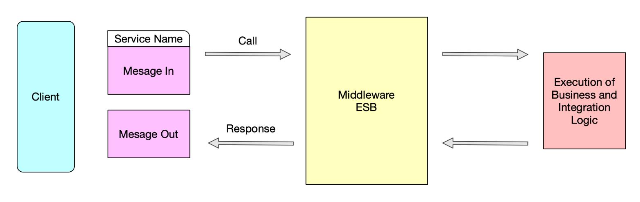
\includegraphics[width=\linewidth]{fig/synchronous_service_call.png}
    \label{fig:Synchronous service call}
\end{figure}

\subsubsection{Asynchronous service call}
\begin{enumerate}
    \item I client compilano i Message In
    \item Il service broker ritorna immediatamente il Communication ID e aggiunge il servizio alla Service Queue
    \item Quando arriva il momento dell'esecuzione, il Service Broker invia l'esecuzione a l'Application Server corretto
    \item Il client può verificare lo stato di esecuzione utilizzando il Communication ID
    \item Il client può ottenere i risultati dell'esecuzione quando lo stato è DONE utilizzando il communicationID e interrogando la ServiceQueue per estrarre il messageOut
\end{enumerate}

\begin{figure}[htp]
    \centering
    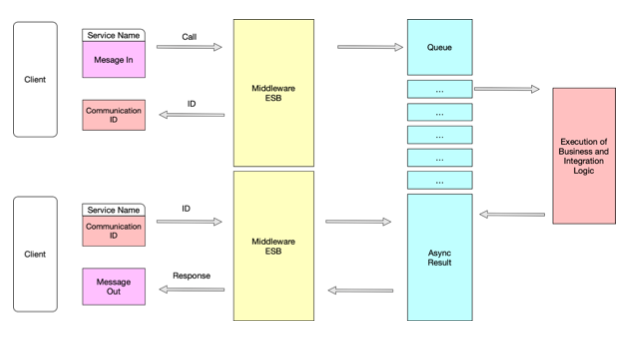
\includegraphics[width=\linewidth]{fig/asynchronous_service_call.png}
    \label{fig:Asynchronous service call}
\end{figure}

\subsubsection{Stream Outbound File Reference}
\begin{enumerate}
    \item Stream Outbound File Reference model è un'estensione degli Async services
    \item Può essere utilizzato quando verrà generato un output di grandi dimensioni
    \item La stessa strategia del CommunicationID viene utilizzata per verificare lo stato
    \item Inoltre un ReferenceID consente al client di aprire il flusso verso il file creato
\end{enumerate}

\begin{figure}[htp]
    \centering
    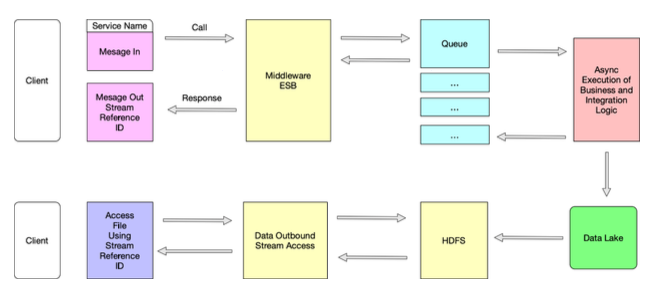
\includegraphics[width=\linewidth]{fig/stream_outbound_file_reference.png}
    \label{fig:Stream Outbound File Reference}
\end{figure}

\subsubsection{Pub/Sub Service Call-back}
\begin{enumerate}
    \item Pub/Sub consente ai clienti di iscriversi a un topic e di ricevere una callback quando si verifica un nuovo evento sul topic sottoscritto
    \item L'ESB nasconde la complessità del Message Bus (Apache Kafka) per semplificare la vita del client
    \item Ogni volta che si verifica un nuovo evento, l'ESB chiama la callback del client fornendo un ObjectID
    \item Il client può ora utilizzare l'ObjectID fornito per ottenere nuovi dati
\end{enumerate}

\begin{figure}[htp]
    \centering
    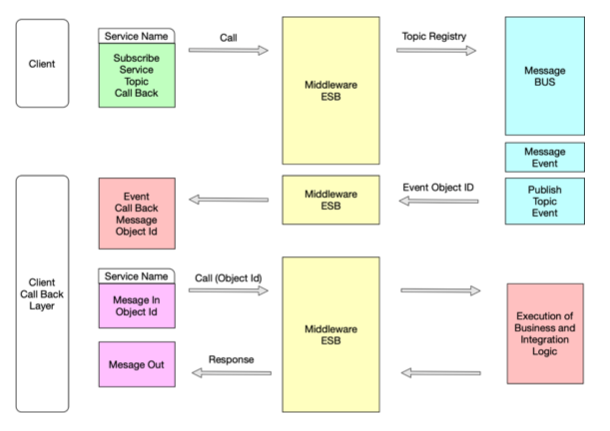
\includegraphics[width=\linewidth]{fig/pub_sub_service_call_back.png}
    \label{fig:Pub/Sub Service Call-back}
\end{figure}

\subsubsection{Batch Sync Data Process}
\begin{enumerate}
    \item Un CDC Job consente l'estrazione incrementale dei dati batch da qualsiasi sistema legacy
    \item Le nuove righe estratte vengono salvate su Data Lake (o DWH) su un percorso denominato secondo convenzione
    \item Un servizio gateway – Reverse CDC Job – esiste per inoltrare queste estrazioni incrementali sui sistemi di destinazione (ad es. SQL DB tramite MERGE o tramite INSERT, APIs, ...)
\end{enumerate}

\begin{figure}[htp]
    \centering
    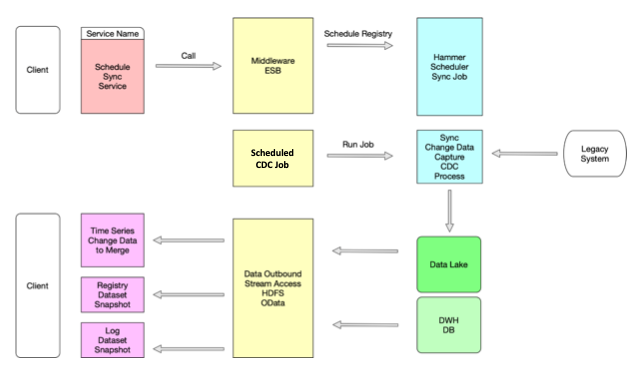
\includegraphics[width=\linewidth]{fig/batch_sync_data_process.png}
    \label{fig:Batch Sync Data Process}
\end{figure}
\section{Project Management}
\subsection{CAPEX vs OPEX}
CAPEX: La spesa in conto capitale (capex o CAPEX) è il denaro speso per acquistare o migliorare un bene fisso, come edifici, veicoli, attrezzature. Il software è considerato una risorsa.

OPEX: Una spesa operativa (opex o OPEX) è un costo continuo per l'esecuzione di un prodotto, un'azienda o un sistema. Le tariffe per la manutenzione del software e le licenze sono costi OPEX.
\subsection{As a Service pattern}
X As A Service si riferisce a qualcosa offerto a qualcuno che nasconde tutta la complessità interna
\begin{itemize}
    \item Infrastructure As A Service consente agli utenti di utilizzare l'HW come se lo possedessero
    \item Software As A Service (ad es. Gmail, Salesforce, ...) offre agli utenti la possibilità di farlo
utilizzare un software senza la necessità di installarlo e mantenerlo
    \item Platform As A Service (ad es. Databricks) consente agli utenti di utilizzare piattaforme complesse per creare la propria applicazione senza preoccuparsi di configurazioni e gestioni complesse
\end{itemize}
\subsection{Make or Buy}

\begin{figure}[htp]
    \centering
    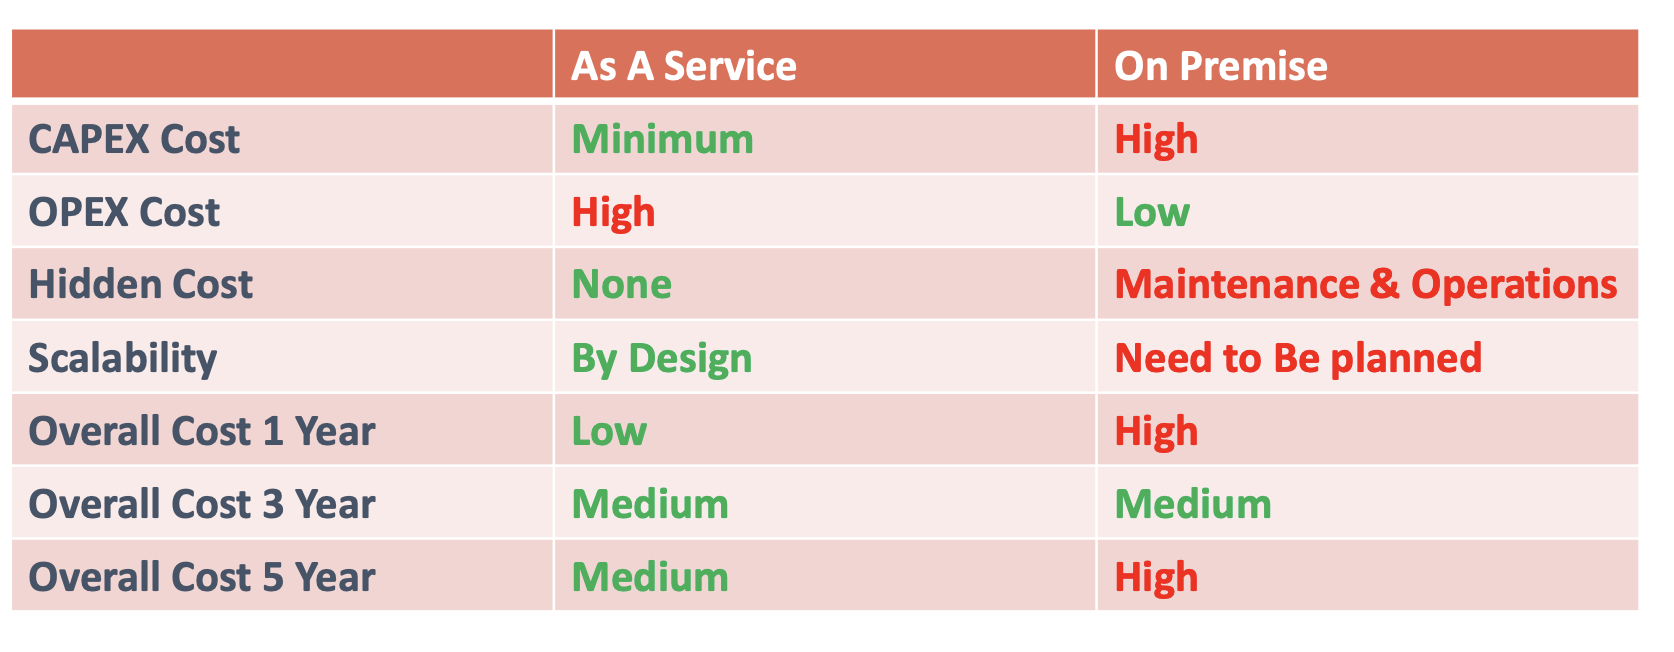
\includegraphics[width=\linewidth]{fig/make_or_buy.png}
    \label{fig:Make Or Buy}
\end{figure}

\subsection{GANTT vs Agile}



\end{document}
